%%%%%%%%%%%%%%%%%%%%%%%%%%%%%%%%%%%%%%%%%
% Simple Sectioned Essay Template
% LaTeX Template
%
% This template has been downloaded from:
% http://www.latextemplates.com
%
% Note:
% The \lipsum[#] commands throughout this template generate dummy text
% to fill the template out. These commands should all be removed when 
% writing essay content.
%
%%%%%%%%%%%%%%%%%%%%%%%%%%%%%%%%%%%%%%%%%

%----------------------------------------------------------------------------------------
%	PACKAGES AND OTHER DOCUMENT CONFIGURATIONS
%----------------------------------------------------------------------------------------

\documentclass[12pt]{article} % Default font size is 12pt, it can be changed here

\usepackage[brazil]{babel}
\usepackage[utf8]{inputenc}
\usepackage{geometry} % Required to change the page size to A4
\geometry{a4paper} % Set the page size to be A4 as opposed to the default US Letter

\usepackage{graphicx} % Required for including pictures

\usepackage{float} % Allows putting an [H] in \begin{figure} to specify the exact location of the figure
\usepackage{wrapfig} % Allows in-line images such as the example fish picture

\usepackage{lipsum} % Used for inserting dummy 'Lorem ipsum' text into the template

\linespread{1.2} % Line spacing

%\setlength\parindent{0pt} % Uncomment to remove all indentation from paragraphs

\graphicspath{{Pictures/}} % Specifies the directory where pictures are stored

\begin{document}

%----------------------------------------------------------------------------------------
%	TITLE PAGE
%----------------------------------------------------------------------------------------

\begin{titlepage}

\newcommand{\HRule}{\rule{\linewidth}{0.5mm}} % Defines a new command for the horizontal lines, change thickness here

\center % Center everything on the page

\textsc{\LARGE Universidade Federal de Pelotas}\\[1.5cm] % Name of your university/college
%\textsc{\Large Keeping a Beat on the Heart}\\[0.5cm] % Major heading such as course name
%\textsc{\large Arrhythmia Monitoring System (AMS)}\\[0.5cm] % Minor heading such as course title

\HRule \\[0.4cm]
{ \huge \bfseries Arrhythmia Monitoring System (AMS)}\\[0.4cm] % Title of your document
\HRule \\[1.5cm]

\begin{minipage}{0.4\textwidth}
\begin{flushleft} \large
\emph{Author:}\\
Alexandre Costa % Your name
\end{flushleft}
\end{minipage}

\vfill % Fill the rest of the page with whitespace

\end{titlepage}

%----------------------------------------------------------------------------------------
%	TABLE OF CONTENTS
%----------------------------------------------------------------------------------------

\tableofcontents % Include a table of contents

\newpage % Begins the essay on a new page instead of on the same page as the table of contents 

%----------------------------------------------------------------------------------------
%	ABISTRACT
%----------------------------------------------------------------------------------------

\section{Abstract} % Major section

In the scope of ubiquitous computing, one of the key issues is the awareness of context, which includes diverse aspects of the user’s situation including his activities, physical surroundings, location, emotions and social relations, device and network characteristics and their interaction with each other. This contextual knowledge is typically acquired from physical, virtual or logical sensors. To overcome problems of heterogeneity and hide complexity, a significant number of middleware approaches have been proposed for systematic and coherent access to manifold context parameters. These frameworks deal particularly with context representation, context management and reasoning, i.e. deriving abstract knowledge from raw sensor data. This article surveys not only related work in these three categories but also the required evaluation principles.

Index Terms—Middleware, Context Provisioning, Context Management, Context Representation, Evaluation, Simulation, Ubiquitous Computing.


%----------------------------------------------------------------------------------------
%	RESUMO
%----------------------------------------------------------------------------------------

\section{Resumo} % Major section

No âmbito da computação ubíqua, uma das questões-chaves é a consciência do contexto, que inclui diversos aspectos da situação do usuário, incluindo suas atividades, ambiente físico, localização, emoções e relações sociais, dispositivos e características da rede e sua interação uns com os outros . Este conhecimento contextual é geralmente adquirido a partir de sensores físicos, virtuais ou lógica. Para superar os problemas de heterogeneidade e de complexidade ocultar, um número significativo de abordagens de middleware têm sido propostos para o acesso sistemática e coerente com os parâmetros de contexto múltiplas. Estes quadros lidar especialmente com a representação contexto, gerenciamento de contexto e de raciocínio, ou seja, decorrentes do conhecimento abstrato a partir dos dados brutos do sensor. Este artigo examina não só o trabalho relacionado nestas três categorias, mas também os princípios de avaliação necessários.

Palavras-chave: Middleware, Provisioning contexto, gestão de contexto, representação, avaliação, simulação de contexto, Computação Ubíqua.

%----------------------------------------------------------------------------------------
%	INTRODUÇÃO
%----------------------------------------------------------------------------------------

\section{Introdução} % Major section

%Ubiquitous Computing (UbiComp) paraphrases the paradigm of hardware and software components being transparently interwoven by means of wireless communication. Value added computer intelligence resulting from the smart and autonomous networking of multiple devices has much more potential than that originating from a single, isolated device. A key objective of these systems is to significantly simplify Human Computer Interaction (HCI) by deploying sensors, processors and actuators in the fabric of everyday life, such that their presence and complexity is hidden from users [1]. UbiComp is commonly understood as the next wave of an evolution chain of computing paradigms, which have gone through the personal computing (second generation) and distributed computing (third generation) from the roots of mainframe computing. Figure 1 illustrates our view of this evolution and highlights some of the features pertinent to the realisation of UbiComp.

Ubiquitous Computing (UbiComp) parafraseia o paradigma de componentes de software que está sendo transparente interligados por meio de comunicação sem fio e hardware. Valor acrescentado inteligência computacional resultante da rede inteligente e autônoma de vários dispositivos tem muito mais potencial do que o proveniente de um único dispositivo, isolado. Um dos principais objetivos destes sistemas é o de simplificar significativamente Interação Humano-Computador (IHC), implantando sensores, processadores e atuadores no tecido da vida cotidiana, de modo que a sua presença e complexidade está escondida dos usuários [1]. UbiComp é comumente entendido como a próxima onda de uma cadeia de evolução dos paradigmas de computação, que passaram a computação pessoal (segunda geração) e computação distribuída (terceira geração) a partir das raízes da computação em mainframe. A figura 1 ilustra a nossa visão dessa evolução e destaca algumas das características pertinentes para a realização de UbiComp.

%------------------------------------------------

\subsection{Context and Context-awareness} % Sub-section

Context is information about a location, its environmental attributes (e.g. noise level, light intensity, temperature, and motion) and the people, devices, objects and software agents that it contains. Context may also include system capabilities, services offered and sought, the activities and tasks in which people and computing entities are engaged, and their situational roles, beliefs, and intentions. Context-awareness is one of the key enablers to facilitate proactive support of users in their current situation. Users do not have to define their situation explicitly by utilising time consuming and counter-intuitive input devices but it is implicitly recognised by the “smart” environment instead. The idea that computing devices can sense and react to stimuli from users’ environment is labelled as context-aware computing.

\begin{figure}[H]
\center{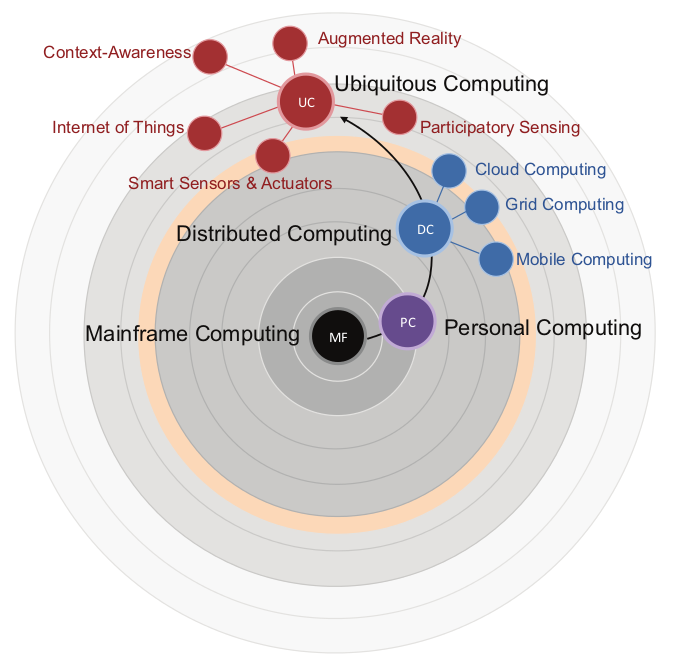
\includegraphics[width=0.5\linewidth]{figura1}}
\caption{Evolution Chain and Features of Ubiquitous Computing.}
\label{fig:speciation}
\end{figure}


%----------------------------------------------------------------------------------------
%	BIBLIOGRAPHY
%----------------------------------------------------------------------------------------

%\begin{thebibliography}{99} % Bibliography - this is intentionally simple in this template

%\bibitem[Figueredo and Wolf, 2009]{Figueredo:2009dg}
%Figueredo, A.~J. and Wolf, P. S.~A. (2009).
%\newblock Assortative pairing and life history strategy - a cross-cultural
%  study.
%\newblock {\em Human Nature}, 20:317--330.
 
%\end{thebibliography}

%----------------------------------------------------------------------------------------

\end{document}

